\documentclass[6pt,letter]{article}\usepackage[]{graphicx}\usepackage[]{color}
% maxwidth is the original width if it is less than linewidth
% otherwise use linewidth (to make sure the graphics do not exceed the margin)
\makeatletter
\def\maxwidth{ %
  \ifdim\Gin@nat@width>\linewidth
    \linewidth
  \else
    \Gin@nat@width
  \fi
}
\makeatother

\definecolor{fgcolor}{rgb}{0.345, 0.345, 0.345}
\newcommand{\hlnum}[1]{\textcolor[rgb]{0.686,0.059,0.569}{#1}}%
\newcommand{\hlstr}[1]{\textcolor[rgb]{0.192,0.494,0.8}{#1}}%
\newcommand{\hlcom}[1]{\textcolor[rgb]{0.678,0.584,0.686}{\textit{#1}}}%
\newcommand{\hlopt}[1]{\textcolor[rgb]{0,0,0}{#1}}%
\newcommand{\hlstd}[1]{\textcolor[rgb]{0.345,0.345,0.345}{#1}}%
\newcommand{\hlkwa}[1]{\textcolor[rgb]{0.161,0.373,0.58}{\textbf{#1}}}%
\newcommand{\hlkwb}[1]{\textcolor[rgb]{0.69,0.353,0.396}{#1}}%
\newcommand{\hlkwc}[1]{\textcolor[rgb]{0.333,0.667,0.333}{#1}}%
\newcommand{\hlkwd}[1]{\textcolor[rgb]{0.737,0.353,0.396}{\textbf{#1}}}%
\let\hlipl\hlkwb

\usepackage{framed}
\makeatletter
\newenvironment{kframe}{%
 \def\at@end@of@kframe{}%
 \ifinner\ifhmode%
  \def\at@end@of@kframe{\end{minipage}}%
  \begin{minipage}{\columnwidth}%
 \fi\fi%
 \def\FrameCommand##1{\hskip\@totalleftmargin \hskip-\fboxsep
 \colorbox{shadecolor}{##1}\hskip-\fboxsep
     % There is no \\@totalrightmargin, so:
     \hskip-\linewidth \hskip-\@totalleftmargin \hskip\columnwidth}%
 \MakeFramed {\advance\hsize-\width
   \@totalleftmargin\z@ \linewidth\hsize
   \@setminipage}}%
 {\par\unskip\endMakeFramed%
 \at@end@of@kframe}
\makeatother

\definecolor{shadecolor}{rgb}{.97, .97, .97}
\definecolor{messagecolor}{rgb}{0, 0, 0}
\definecolor{warningcolor}{rgb}{1, 0, 1}
\definecolor{errorcolor}{rgb}{1, 0, 0}
\newenvironment{knitrout}{}{} % an empty environment to be redefined in TeX

\usepackage{alltt} 

%%%%%%%%%%%%%%%%%%%%
%%%%%% Package %%%%%
%%%%%%%%%%%%%%%%%%%%

%\usepackage[latin1]{inputenc}
\usepackage[parfill]{parskip} % Activate to begin paragraphs with an empty line rather than an indent
\usepackage{amsmath,amsthm,amssymb,bbm} %math stuff
\usepackage{placeins} % FloatBarrier
\usepackage{fancyhdr}
\usepackage{lastpage}
\usepackage{float}    % for fig.pos='H'
%\usepackage{subfig}   % for subfigure
\usepackage{subcaption}  % an alternative package for sub figures
\usepackage{comment}
\bibliographystyle{plainnat}
\usepackage{setspace} %Spacing
\usepackage{graphicx,graphics}
\usepackage{booktabs,tabularx}
\usepackage{enumerate}
\usepackage{makecell}
\usepackage{xfrac}
\restylefloat{figure}
\usepackage{appendix}
\usepackage{color, colortbl, xcolor}
\usepackage{booktabs,dcolumn} % for use with texreg in R
\usepackage[bookmarks]{hyperref}
\usepackage[numbers]{natbib}
\bibliographystyle{ksfh_nat}
\usepackage{wrapfig}
\usepackage{todonotes}
\usepackage{fancyvrb}



%%%%%%%%%%%%%%%%%%%%%%%%%
%%%%%% Configuration %%%%
%%%%%%%%%%%%%%%%%%%%%%%%%

\newcommand{\nd}{\noindent}
\newcommand{\ntodo}[2][]{\todo[#1]{\thesubsubsection{}. #2}}

% Define the format of the report
\renewcommand{\headrulewidth}{0.0pt}
\renewcommand{\footrulewidth}{0.0pt}
\setlength{\textheight}{9.00in}
\setlength{\textwidth}{7.00in}
\setlength{\topmargin}{-0.5in}
\setlength{\evensidemargin}{-0.25in}
\setlength{\oddsidemargin}{-0.25in}
\renewcommand{\baselinestretch}{1.2}
\makeatletter
\makeatother
\lfoot{} \cfoot{ } \rfoot{{\small{\em Page \thepage \ of \pageref{LastPage}}}}

\newenvironment{conditions}
  {\par\vspace{\abovedisplayskip}\noindent\begin{tabular}{>{$}l<{$} @{${}={}$} l}}
  {\end{tabular}\par\vspace{\belowdisplayskip}}
%%%%%%%%%%%%%%%%%%%%%%%%%%%%%%%%%%%%%%%%%%%%%%%%%%%
%%%%%%%%%%%%%%%%% BEGIN        %%%%%%%%%%%%%%%%%%%%
%%%%%%%%%%%%%%%%%%%%%%%%%%%%%%%%%%%%%%%%%%%%%%%%%%%
\IfFileExists{upquote.sty}{\usepackage{upquote}}{}
\begin{document}
\pagestyle{plain}
\pagenumbering{gobble}

\title{%
 Méthodes avancées en exploitation de donnée \\
  \large (MATH80619)}
\author{\begin{tabular}{ll}
    Estefan Apablaza-Arancibia & 11271806\\
        Adrien Hernandez & 11269225\\

    
\end{tabular}}
\maketitle
\newpage
\pagestyle{plain}


%%%%%%%%%%%%%%%%%%%%%%%%%%%%%%%%%%%%%%%%%%%%%%%%%%%
%%%%%%%%%%%%%%%%% INTRODUCTION %%%%%%%%%%%%%%%%%%%%
%%%%%%%%%%%%%%%%%%%%%%%%%%%%%%%%%%%%%%%%%%%%%%%%%%%
\newpage
\pagestyle{fancy}
\pagenumbering{arabic}
\section{Introduction}
In the first section of this paper, a literature review covers the neural networks and deep learners algorithms, focusing on different type of neural networks architecture; the purpose of adding multiple hidden layers and, ultimately, what are the challenges regarding the increase in computing time. Furthermore, in the methodology section, a list of deep learning projects are shown in order to understand some patterns and methods. Then, an exhaustive list of the R libraries allowing to build neural networks and deep learners models. Correspondingly, the advantages and disadvantages of each libraries, their capabilities as well as what you can expect when using them. To sum up, the last section will give concrete examples on how to implement the neural networks and deep learners models with these libraries, using real data.

%%%%%%%%%%%%%%%%%%%%%%%%%%%%%%%%%%%%%%%%%%%%%%%%%%%
%%%%%%%%%%%%%%%%%% Litterature %%%%%%%%%%%%%%%%%%%%
%%%%%%%%%%%%%%%%%% Review      %%%%%%%%%%%%%%%%%%%%
%%%%%%%%%%%%%%%%%%%%%%%%%%%%%%%%%%%%%%%%%%%%%%%%%%%

\section{Litterature Review}
\subsection{What is Deep Learning and why use it?}
\begin{wrapfigure}[14]{r}{0.5\textwidth}
  \begin{center}
    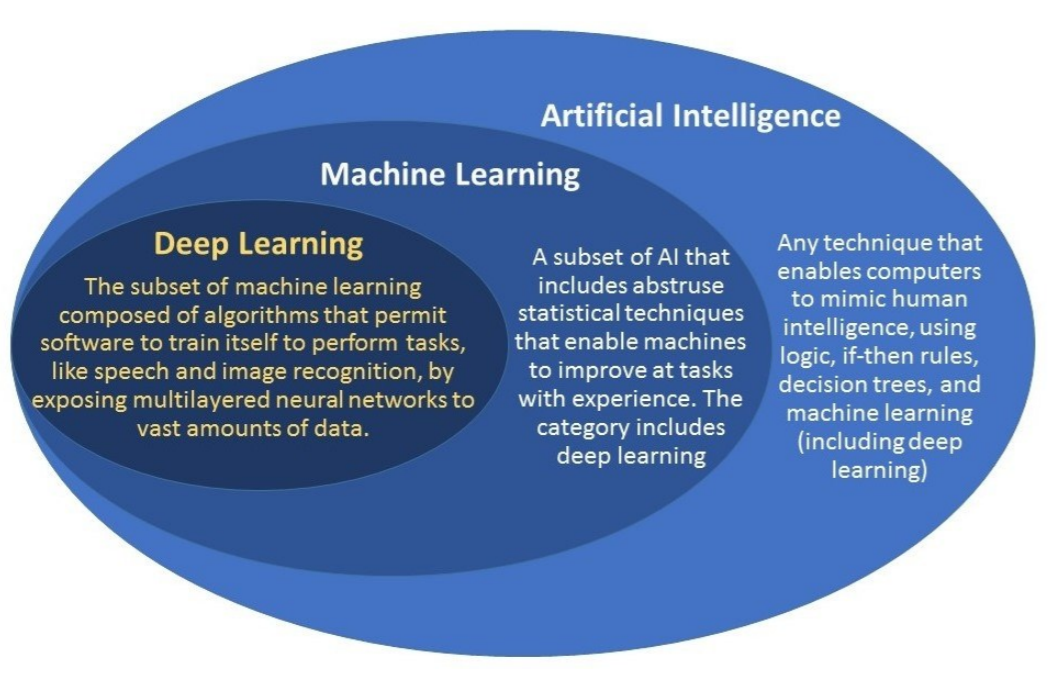
\includegraphics[width=0.4\textwidth]{figure/deep learning.PNG}
      \end{center}
     \caption{Artificial Intelligence vs Machine Learning vs Deep Learning}
     \label{fig:simule}
\end{wrapfigure}

Deep learning is a subset field of articial intelligence and can be seen as a specific way of doing machine learning. Deep learning algorithms can be seen as feature representation learning. Indeed, by applying to the data multiple non-linear transformations through the use of hidden layers, deep learning models have their own trainable feature extration capability making it possible to learn specific features from the data without needing a specific human domain expert. This means that deep learning models won't require the features extraction step that is essential for classic machine learning models. However, increasing the models capacity by adding hidden layers, requires increasingly computing power and slow down the training process of the model. The choice of hyperparameters, programming languages and memory management will therefore be important criteria to take into account while building deep learning models\\
Since the last decade, deep learning models have shown notable predictive power and have been revolutionizing an important number of domain such as computer vision, natural language understanding, fraud detection, health and much more.\\
As a first glance in the subject, it is highly recommended it to read  a reference from pioneers in the field (\cite[Chapter 1]{Goodfellow-et-al-2016}).


\subsubsection{Feed Forward Neural Network}
\begin{wrapfigure}[12]{R}{0.5\textwidth}
  \begin{center}
    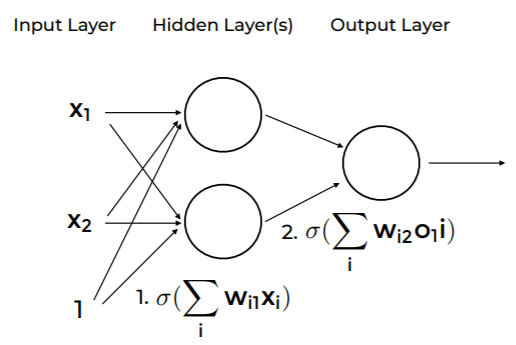
\includegraphics[width=0.4\textwidth]{figure/feedforward_neural_networks.png}
  \end{center}
  \caption{feedforward neural networks}
  \label{fig:attention}
\end{wrapfigure}

"Deep feedforward networks, also called feedforward neural networks, or multilayer perceptrons (MLPs), are the quintessential deep learning models." \cite{Goodfellow-et-al-2016}

FNN models are inspired from biology and by the way the human brain works. In a neural network, each neuron takes input from other neurons, processes the information and then transmits outputs to next neurons. Artificial neural networks follow the same process as each neuron will perform the weighted sum of inputs and will add a bias as a degree of freedom. It will then apply a non-linear transformation before outputting the information. Thus, the information goes forward in the network; neurons transmit information from the input layers towards the output layer. It is important to know that in a feedfoward neural networks (fig. \ref{fig:attention}) the neurons of a same layer are not connected to each other; they do not allow any feedback connections within a same layer. If we want to allow this process, we will be looking at recurrent neural networks.

The equation a neuron input is  
\begin{equation}
a(x) = b +\sum_{i}{w_i x_i}
\end{equation}
and the output
\begin{equation}
h(x) = g(a(x))
\end{equation}
where:
\begin{conditions}
 x     &  the input data \\
 b     &  the bias term \\
 w     &  the weight or parameter \\   
 g(...) &  the activation function
\end{conditions}

Here, \textbf{the bias term  b} and \textbf{the weights or parameter w} will be learned by the model in order the minimize a cost function, through the use of the gradient descent method. Then, the network will use the backpropagation algorithm where the error is backpropagated from the output to the input layers and the bias and weighted are then updated accordingly.\\
Regarding the \textbf{activation function g(...)}, the common practice is to use a ReLu (rectified linear unit) as the activation function for the neurons of the hidden layers. Regarding the neurons of the last layer, the activation function will be chosen accordingly to the task we want our model to perform:\\
\begin{figure}[h]
    \centering
    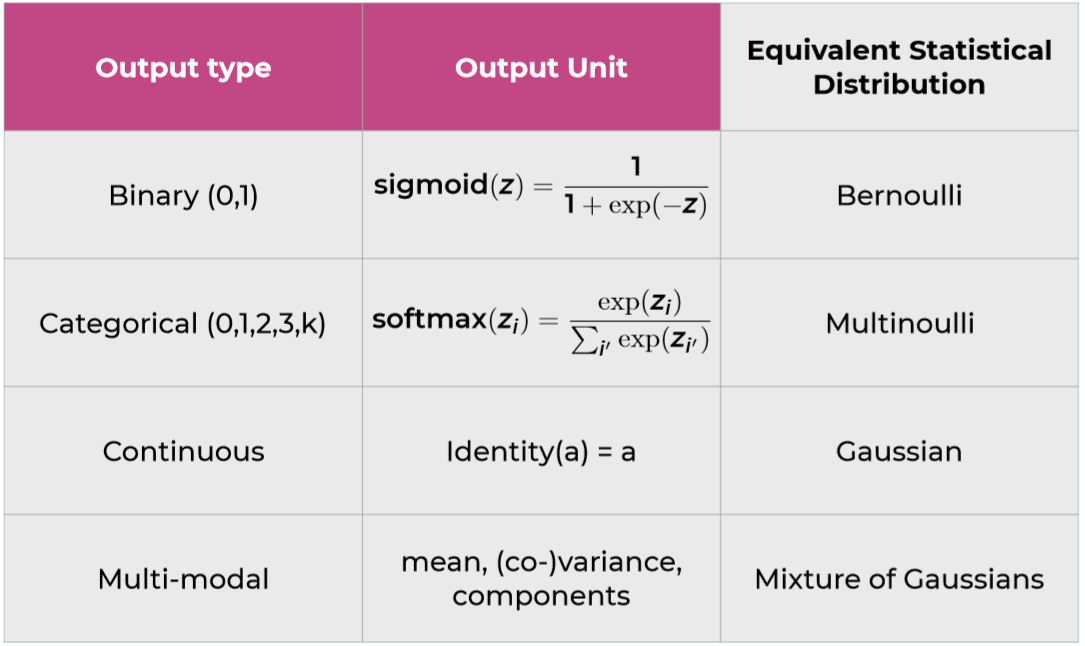
\includegraphics[width=0.45\textwidth]{figure/activation_function_output.png}
     \caption{Activation functions: output units. HEC}
     \label{fig:activation}
\end{figure}

A detailed explanation of the theory of feedforward neural network can be found in \cite[Chapter 6]{Goodfellow-et-al-2016}

\subsubsection{CNN}

The CNN are a modified architecture of FNN that leverage the feature engineering that used to be hand maded by domain experts. This class of deep neural network are commonly use for image recognition and classification that can serve different applications such as facial recongnition, document analysis and speech recognition. The original FNN are not suited analyzing large size images since the weights increase exponentially and, at the end, don't perfom very well.\\
\begin{wrapfigure}[12]{r}{0.5\textwidth}
  \begin{center}
    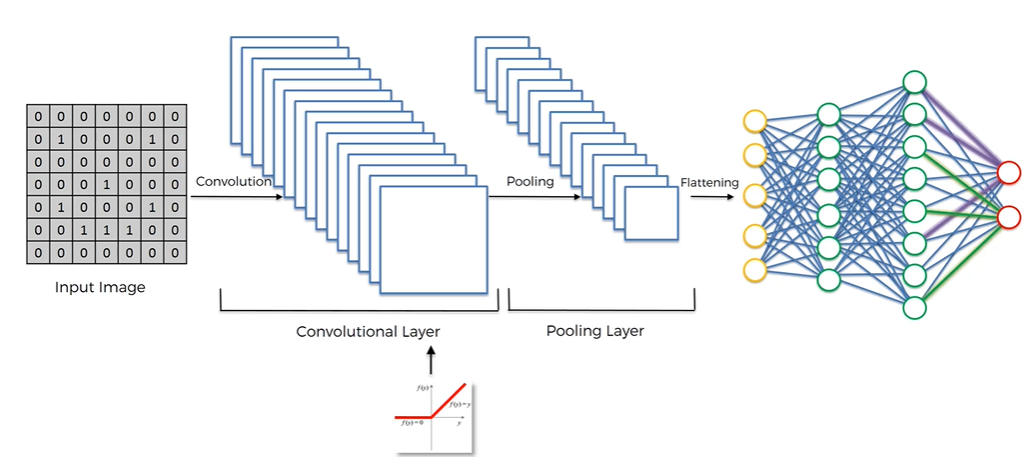
\includegraphics[width=0.5\textwidth]{figure/CNN_process.png}
  \end{center}
  \caption{CNN, Deep Learning A-Z by SuperDataScience}
  \label{fig:attention}
\end{wrapfigure}
A standard architecture of a CNN model is commonly represented this way: We start with an input image to which we are going to apply several kernels, a.k.a features detectors, in order to create feature maps that will form what we call a convolutional layer. A common practice is to apply the ReLu activation fonction to the convolutional layer output in order to increase the non linearity of the images before using the pooling method to create a pooling layer. The next step will be to combine all the pooled images from the pooling layer into one single vector, which is called flattening and will be the input of a FNN that will perform the desired task, for instance, classification. CNN parameters are trained with the backpropagation algorithm where the gradients are propagated from the output layer of the FFN to the input of the CNN in order to minimise a cost function, most of the time a categorical cross-entropy if we are performing a multi-class classification. 


To get a detailed explanation of convolutional neural networks we recommand to read \cite[Chapter 9]{Goodfellow-et-al-2016}.\\

\subsubsection{RNN}
Recurrent neural networks are a more advanced type of neural networks architecture having proven state-of-art performance for solving tasks related to sequential data such as Natural Language Processing (NLP), anomaly detection and event forecasting. As a key differentiator from feedfoward neural networks, is that RNNs use feedback loops connections instead of feedforward connections and get an internal memory. Indeed, that take as input each step of the sequantial data as well as what they have learned over time. One of their other advantage is to be able to handle input and ouput sequences with different sizes. "A recurrent neural network can be thought of as multiple copies of the same network, each passing a message to a successor" Olah.
\begin{figure}[h]
    \centering
    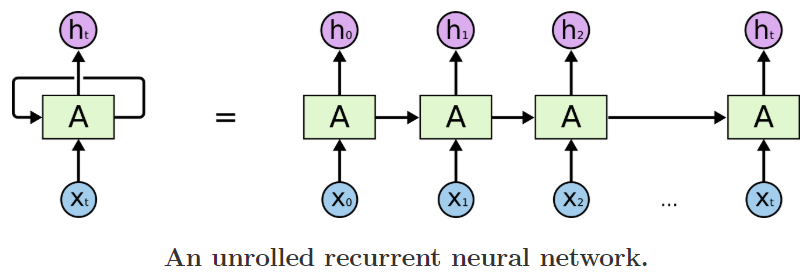
\includegraphics[width=0.45\textwidth]{figure/RNN_process.png}
     \caption{RNN, Understanding LSTM Networks by Olah}
     \label{fig:rnn_process}
\end{figure}

To get a detailed explanation of the theory of recurrent neural networks we recommand to read \cite[Chapter 10]{Goodfellow-et-al-2016}. We also recommand reading this blog post \url{https://colah.github.io/posts/2015-08-Understanding-LSTMs/}

\subsection{How to integrate Deep Learning in R}
The integration of Deep learning in R can be separate in two part ; (1) The API integration and (2) the standalone R packages. 
\begin{enumerate}
\item The API will give the possibility to control externally through R an existing installation. In other words, a software translator for a already known software installation. This approach is not always trivial to install nor to manipulate but in long term will probably give the best flexibility in terms of Deep Learning projects.
\item The standalone R packages will be packages that require no third party software in order to create the deep learning projects. This approach is relatively fast to install but is restraing in terms deep learning architecture.
\end{enumerate}
A list of the available resources with installation and examples tutorials can be found in section \ref{avail_ressour} and \ref{examples} .

%%%%%%%%%%%%%%%%%%%%%%%%%%%%%%%%%%%%%%%%%%%%%%%%%%%
%%%%%%%%%%%%%%%%%% Description %%%%%%%%%%%%%%%%%%%%
%%%%%%%%%%%%%%%%%% of methods  %%%%%%%%%%%%%%%%%%%%
%%%%%%%%%%%%%%%%%%%%%%%%%%%%%%%%%%%%%%%%%%%%%%%%%%%
\section{Methodology}
This section is divided in two;  the dataset description and the benchmark type. The dataset description is mostly to describe what dataset is going to be use for the different type of deep learning algorithms. The second section will describe two indicators in order to compare results of similar algorithms. The first indicator is mostly about a simple accuracy base on the same training and validation dataset and second indicator is about the time it took to execute the same task on differents ressources.
\subsection{Dataset}
\subsubsection{FNN}
For the FNN, the training data will be the well known \textit{Iris} dataset. It contains four covariables and one categorical target variable.


\begin{knitrout}
\definecolor{shadecolor}{rgb}{0.969, 0.969, 0.969}\color{fgcolor}\begin{kframe}
\begin{alltt}
\hlkwd{library}\hlstd{(datasets)}
\hlstd{library}
\hlkwd{data}\hlstd{(iris)}
\hlkwd{set.seed}\hlstd{(}\hlnum{123}\hlstd{)}
\hlstd{iris}\hlopt{$}\hlstd{Species} \hlkwb{=} \hlkwd{sapply}\hlstd{(}\hlkwd{as.character}\hlstd{(iris}\hlopt{$}\hlstd{Species),}
                      \hlstd{switch,} \hlstr{"setosa"} \hlstd{=} \hlnum{1}\hlstd{,} \hlstr{"versicolor"} \hlstd{=} \hlnum{2}\hlstd{,} \hlstr{"virginica"} \hlstd{=} \hlnum{3}\hlstd{,} \hlkwc{USE.NAMES} \hlstd{= F)}
\hlstd{spec} \hlkwb{=} \hlkwd{c}\hlstd{(}\hlkwc{train} \hlstd{=} \hlnum{.7}\hlstd{,}\hlkwc{test} \hlstd{=} \hlnum{.3}\hlstd{)}
\hlstd{g} \hlkwb{=} \hlkwd{sample}\hlstd{(}\hlkwd{cut}\hlstd{(}\hlkwd{seq}\hlstd{(}\hlkwd{nrow}\hlstd{(iris)),}\hlkwd{nrow}\hlstd{(iris)}\hlopt{*}\hlkwd{cumsum}\hlstd{(}\hlkwd{c}\hlstd{(}\hlnum{0}\hlstd{,spec)),}\hlkwc{labels} \hlstd{=} \hlkwd{names}\hlstd{(spec)))}
\hlstd{data_df} \hlkwb{=} \hlkwd{split}\hlstd{(iris, g)}
\hlstd{X} \hlkwb{=} \hlkwd{c}\hlstd{()}
\hlstd{Y} \hlkwb{=} \hlkwd{c}\hlstd{()}
\hlstd{X}\hlopt{$}\hlstd{train} \hlkwb{=} \hlkwd{as.matrix}\hlstd{(data_df}\hlopt{$}\hlstd{train[,}\hlopt{-}\hlkwd{ncol}\hlstd{(data_df}\hlopt{$}\hlstd{train)])}
\hlstd{X}\hlopt{$}\hlstd{test} \hlkwb{=} \hlkwd{as.matrix}\hlstd{(data_df}\hlopt{$}\hlstd{test[,}\hlopt{-}\hlkwd{ncol}\hlstd{(data_df}\hlopt{$}\hlstd{test)])}
\hlstd{Y}\hlopt{$}\hlstd{train} \hlkwb{=} \hlkwd{as.matrix}\hlstd{(data_df}\hlopt{$}\hlstd{train[,}\hlkwd{ncol}\hlstd{(data_df}\hlopt{$}\hlstd{train)])}
\hlstd{Y}\hlopt{$}\hlstd{test} \hlkwb{=} \hlkwd{as.matrix}\hlstd{(data_df}\hlopt{$}\hlstd{test[,}\hlkwd{ncol}\hlstd{(data_df}\hlopt{$}\hlstd{test)],)}
\end{alltt}
\end{kframe}
\end{knitrout}

\begin{knitrout}
\definecolor{shadecolor}{rgb}{0.969, 0.969, 0.969}\color{fgcolor}\begin{kframe}
\begin{alltt}
\hlkwd{print}\hlstd{(}\hlkwd{head}\hlstd{(X}\hlopt{$}\hlstd{train))}
\end{alltt}
\begin{verbatim}
##    Sepal.Length Sepal.Width Petal.Length Petal.Width
## 1           5.1         3.5          1.4         0.2
## 2           4.9         3.0          1.4         0.2
## 4           4.6         3.1          1.5         0.2
## 7           4.6         3.4          1.4         0.3
## 8           5.0         3.4          1.5         0.2
## 10          4.9         3.1          1.5         0.1
\end{verbatim}
\begin{alltt}
\hlkwd{print}\hlstd{(}\hlkwd{head}\hlstd{(Y}\hlopt{$}\hlstd{train))}
\end{alltt}
\begin{verbatim}
## [1] 0 0 0 0 0 0
\end{verbatim}
\end{kframe}
\end{knitrout}

\subsubsection{CNN}
For the CNN, the training data will also be a well known dataset called CIFAR-10. The CIFAR-10 dataset consists of 60000 32x32 colour images in 10 classes, with 6000 images per class. The easiest way in R to download this package is using the Keras API. The training dataset has 50 000 images in three color (Red-Green-Blue) that are 32 pixels by 32 pixels. The testing dataset has a total of 10 000 images
\begin{knitrout}
\definecolor{shadecolor}{rgb}{0.969, 0.969, 0.969}\color{fgcolor}\begin{kframe}
\begin{alltt}
\hlkwd{library}\hlstd{(keras)}
\hlstd{cifar10} \hlkwb{=} \hlkwd{dataset_cifar10}\hlstd{()}
\end{alltt}
\end{kframe}
\end{knitrout}

\subsubsection{RNN}
The dataset use to test an RNN is the IMDB Movie reviews sentiment classification. This pack
\begin{knitrout}
\definecolor{shadecolor}{rgb}{0.969, 0.969, 0.969}\color{fgcolor}\begin{kframe}
\begin{alltt}
\hlstd{idmb} \hlkwb{=} \hlkwd{dataset_imdb}\hlstd{(}  \hlkwc{path} \hlstd{=} \hlstr{"imdb.npz"}\hlstd{,} \hlkwc{num_words} \hlstd{=} \hlkwa{NULL}\hlstd{,} \hlkwc{skip_top} \hlstd{=} \hlnum{0L}\hlstd{,} \hlkwc{maxlen} \hlstd{=} \hlkwa{NULL}\hlstd{,}
                      \hlkwc{seed} \hlstd{=} \hlnum{113L}\hlstd{,} \hlkwc{start_char} \hlstd{=} \hlnum{1L}\hlstd{,} \hlkwc{oov_char} \hlstd{=} \hlnum{2L}\hlstd{,} \hlkwc{index_from} \hlstd{=} \hlnum{3L}\hlstd{)}
\end{alltt}
\end{kframe}
\end{knitrout}

\begin{comment}
\subsection{Benchmark}
\subsubsection{Accuracy}
\subsubsection{Time elapsed}
\end{comment}
%%%%%%%%%%%%%%%%%%%%%%%%%%%%%%%%%%%%%%%%%%%%%%%%%%%
%%%%%%%%%%%%%%%%%% Resources   %%%%%%%%%%%%%%%%%%%%
%%%%%%%%%%%%%%%%%% available   %%%%%%%%%%%%%%%%%%%%
%%%%%%%%%%%%%%%%%%%%%%%%%%%%%%%%%%%%%%%%%%%%%%%%%%%

\section{Available resources}
\label{sec:avail_ressour}
Like explain earlier this section will be divided in two in order to really differantiate the R packages standalone of the ressources that add an application interface.
%%%%%%%%%%%%%%%%%%%%%%%%%%%%%%%%%%%%%%%%%%%%%%%%%%%
%%%%%%%%%%%%%%%%%% R Package   %%%%%%%%%%%%%%%%%%%%
%%%%%%%%%%%%%%%%%%%%%%%%%%%%%%%%%%%%%%%%%%%%%%%%%%%
\subsection{R packages}
\ntodo[inline]{à voir si on a encore de la place pour mettre un tableau récapitulatif}

%%%%%%%%%%%%%%%% Neuralnet %%%%%%%%%%%%%%%% 
\subsubsection{Neuralnet package}
\textbf{Keyword: FNN; Deep FNN}
\paragraph{Description}
According to its CRAN description, the package allows the "training of neural networks using the backpropagation, resilient backpropagation with (Riedmiller, 1994) or without weight backtracking (Riedmiller, 1993) or the modified globally convergent version by Anastasiadis et al. (2005). The package allows flexible settings through custom-choice of error and activation function. Furthermore, the calculation of generalized weights (Intrator O \& Intrator N, 1993) is implemented." This package uses $C/C++$ in backend.

\begin{figure}[h]
    \centering
    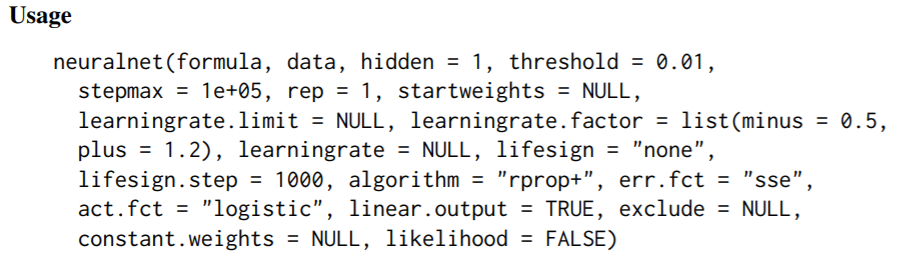
\includegraphics[width=0.7\textwidth]{figure/neuralnet_package.png}
     \caption{Package neuralnet, CRAN}
\end{figure}

\paragraph{Pros}
\begin{itemize}
\item Very easy to use and to build a quick FFN and deep FNN model.
\item Allows to use several types of backpropagation algorithms. By default, the resilient backpropagation algorithm is used "rprop+" instead of regular backpropagation which is an algorithm not very used in practice as it is more tricky to implement. We can however decided to change the rprop+ for a standard backpropagation by changing for \textbf{algorithm = "backprop"}.
\item Several hidden layers and neurons per layer can be added. By default, the algorithm uses only 1 hidden layer with 1 neuron, but it can be increased by addind the command line: \textbf{hidden = c(5,2)} to get 2 hidden layers of 5 neurons.
\item Allows to easily plot and visualize the model and its parameters with the command line: \textbf{plot(model).}
\end{itemize}
\paragraph{Cons}
\begin{itemize}
\item One of the disadvantage of this package is that it requires some data preprocessing as it only works with numeric inputs. Therefore, factor variables will need to be transformed into dummies during the preprocessing phase. 
\item The package doesn't provide built-in normalization functions. Therefore, it is recommended to manually normalize the data before using them as input in the neural networks in order to reduce the number of iretation of the algorithm.
\end{itemize}

%%%%%%%%%%%%%%%% nnet %%%%%%%%%%%%%%%% 
\subsubsection{nnet package}
\textbf{Keyword: FNN}
\paragraph{Description}
This package comes from the CRAN platform and allows to build and fit "FNN with a single hidden layer and multinomial log-linear models". This package uses C/C++ in backend.
\begin{figure}[h]
    \centering
    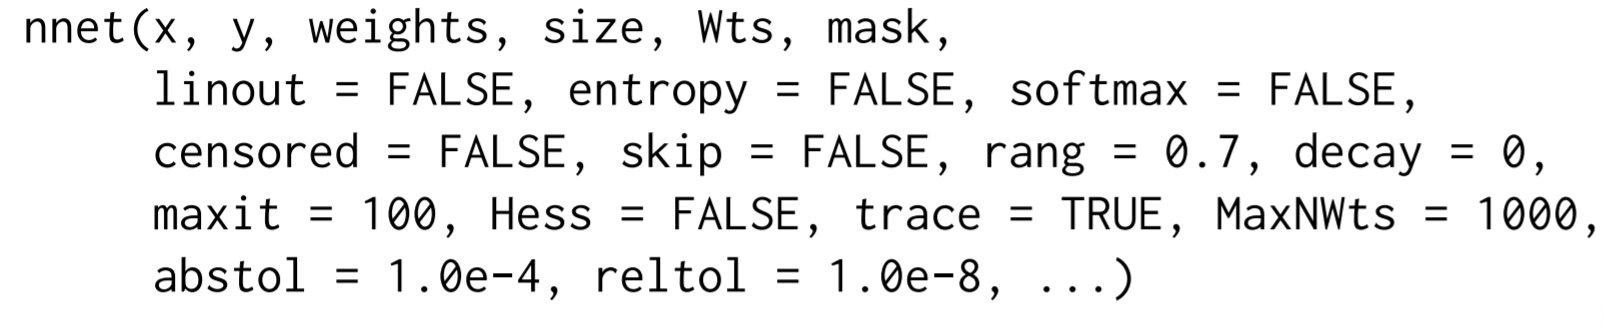
\includegraphics[width=0.45\textwidth]{figure/nnet_package.png}
     \caption{Package nnet, CRAN}
\end{figure}
\paragraph{Pros}
\begin{itemize}
\item One of the easiest R package to build a quick FFN model.
\end{itemize}
\paragraph{Cons}
\begin{itemize}
\item It does not offer a lot of flexibility, and can only apply logistic sifmoid function for the hidden layer activation and cannot use tanH and ReLu.
\item This package does not allow to use more that one hidden layer, and does not have any feature to find the optimal number of neurones in the hidden layer. It is up to the analyst to build a loop to test by cross-validation, for exemple, the optimal hyperparameter values.
\item Cannot use classical backpropagation algorithm to train the network. It only uses the BFGS (Broyden-Fletcher-Goldfarb-Shanno) which is a Quasi-Newton method and therefore increases the number of computation to reach a local optima. However, applied on a small dataset with a model having only one hidden layer does not seem to be a problem.
\item Does not have any function to plot the model.
\end{itemize}

%%%%%%%%%%%%%%%% NeuralNetTools %%%%%%%%%%%%%%%% 

\subsubsection{NeuralNetTools package}
\textbf{Keywords: Visualization; Variable importance; Sensitivity}
\paragraph{Description}
This package is a complement to R's neural networks packages as it allows to visualize and perform analysis on neural network models. "Functions are available for plooting, quantifying variable importance, conducting a sensitivity analysis, and obtaining a simple list of model weights."
\begin{figure}[H]
  \begin{subfigure}{0.5\textwidth}
    \centering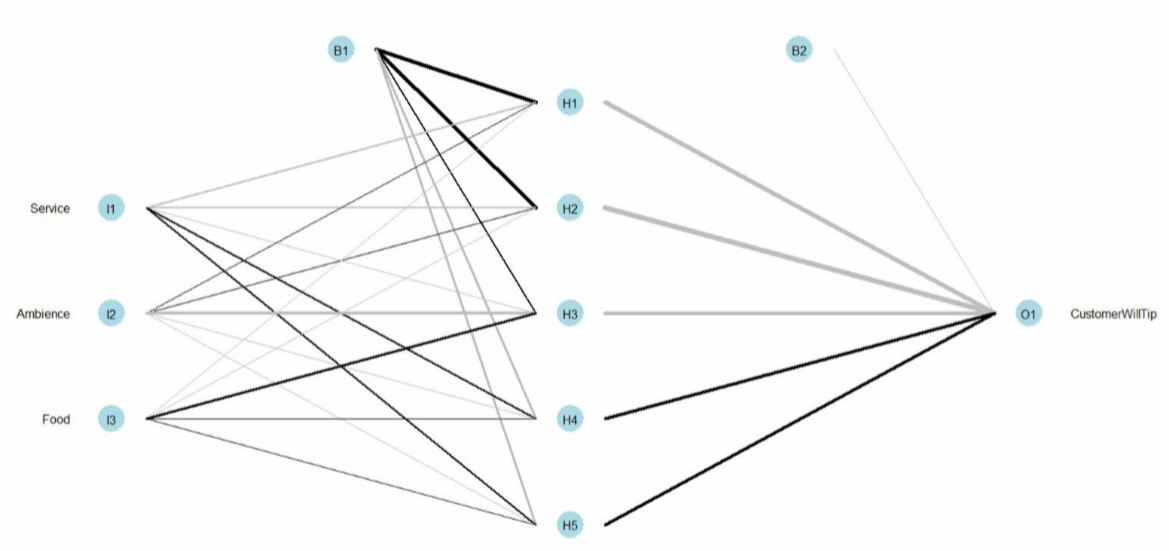
\includegraphics[width=0.45\textwidth]{figure/plotnet.png}
    \caption{NeuralNetTools, plotnet function}
  \end{subfigure}
  \begin{subfigure}{0.5\textwidth}
    \centering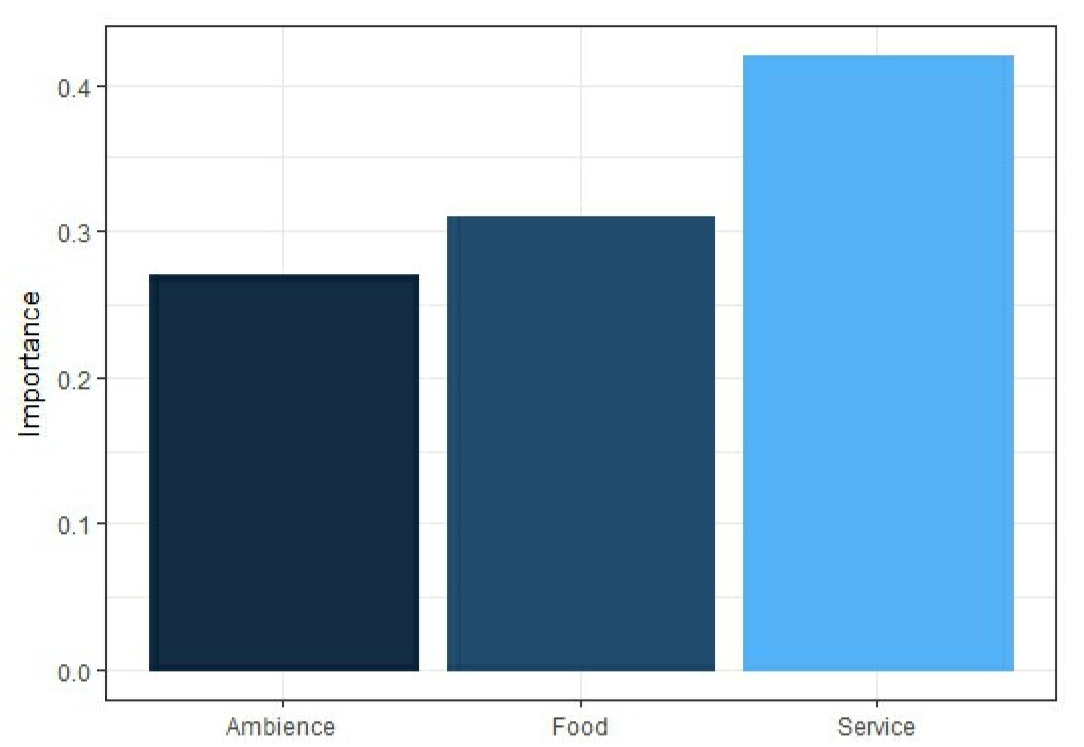
\includegraphics[width=0.45\textwidth]{figure/garson_algorithm.png}
    \caption{NeuralNetToolsm Input variables importance}
  \end{subfigure}
    \caption{Embedding dimension hyper parameter}
\end{figure}

\paragraph{Pros}
\begin{itemize}
\item Very easy to plot your neural network models with the function \textbf{plotnet(model)}.
\item Visualize the input variables importance to the output prediction witht the Garson and olden algorithm.
\item Perform sensitivity analysis on your neural networks model using the Lek profile method.
\item Works with the models built from different packages: \textbf{caret, neuralnet, nnet, RSNSS}
\item Can plot neural networks with pruned connections from the RSNSS package.
\end{itemize}

\paragraph{Cons}
\begin{itemize}
\item Does not provide any function for neural network model development.
\item Is not optimized to visualize large neural networks models.
\end{itemize}



%%%%%%%%%%%%%%%% Deepnet %%%%%%%%%%%%%%%% 
\subsubsection{Deepnet package}
\textbf{Keywords: FNN; RBM; DBN; Autoencoder}
\paragraph{Description}
This package is available on the CRAN platform and has been written specifcally written for R. It allows "implement som deep learning architectures and neural network algorithms, including backpropagation, Restricted Boltzmann Machine (RBM), Deep Belief Network (DBN) and Deep autoencoder".
\begin{figure}[h]
    \centering
    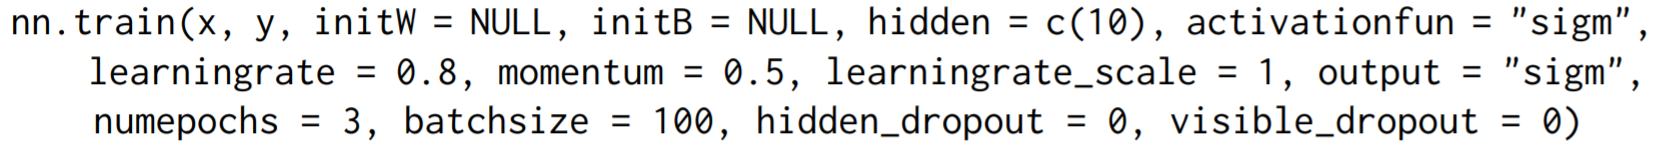
\includegraphics[width=0.7\textwidth]{figure/deepnet_package.png}
     \caption{Package deepnet, CRAN}
\end{figure}
\paragraph{Pros}
\begin{itemize}
\item Allows to load benchmark datasets such as MNIST with the function load.mnist(dir)
\item Allows to initialize the weights of a FNN with the Deep Belief Network algorithm (dbn.dnn.train()) or Stacked AutoEncoder algorithm (sae.dnn.train()).
\item Allows to have an estimation of the probabilistic distribution of a dataset trough the use of the Restricted Boltzmann machine algorithm.
\item Have more activation functions than the other R packages. Hidden Layers activation function can be linear, sigmoid or tanh. The output activation function can be linar, sigmoid or softmax.
\end{itemize}
\paragraph{Cons}
\begin{itemize}
\item Does not support the ReLu activation function for hidden layers.
\item Not the fastest package due to its implementation in R.
\item Does not provide a lot of hyperparameters tuning options, and is not user-friendly.
\end{itemize}


%%%%%%%%%%%%%%%% Nnet %%%%%%%%%%%%%%%% 

%%%%%%%%%%%%%%%% brnn %%%%%%%%%%%%%%%% 
\subsubsection{brnn package}
\textbf{Keywords: Bayesian Regularization; FNN}
\paragraph{Description}
This package available on the platform CRAN, allows to perform "Baeysian regularized neural networks inclusing both additive and dominance effects, and allows to takes advantage of multicore architectures via a parallel computing approach using openMP for the computations". (Pérez-Rodriguez, ...)
\begin{figure}[h]
    \centering
    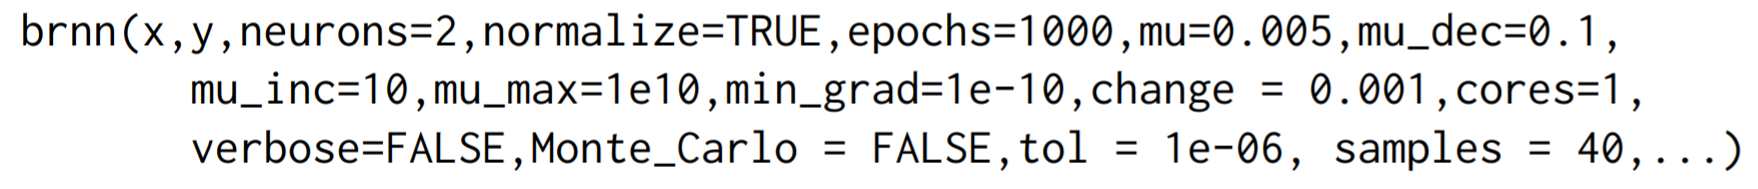
\includegraphics[width=0.45\textwidth]{figure/brnn_package.png}
     \caption{Package nnet, CRAN}
\end{figure}
\paragraph{Pros}
\begin{itemize}
\item Allows to add Additive and Dominance effects in the neural networks models.
\item Take advantage of multicore processors (only for UNIX-like systems).
\item Allows to use a Gauss-Newton algorithm for optimization.
\item The package is able to assign initial weights by using the Nguyen and Widrow algorithm.
\item Include an algorithm to deal with ordinal data by using the function \textbf{brnn\_ordinal(x, ...)}
\item It has a function to normalize and unnormalized the data.
\end{itemize}
\paragraph{Cons}
\begin{itemize}
\item Cannot use the classic backpropagation algorithm for optimization.
\item The package fits a two layers neural networks and it is not possible to increase the number of hidden layers.
\end{itemize}

%%%%%%%%%%%%%%%% rnn %%%%%%%%%%%%%%%% 
\subsubsection{rnn package}
\textbf{Keywords: RNN}
\textbf{Installation:} You will need to install the diges package first through the function \textbf{install.packages(digest)} in order to download the rnn package.
\paragraph{Description}
Avaible from the CRAN platform, this package allows the "implementation of a Recurrent Neural Network architectures in native R, including Long-Short Term Memory (LSTM), Gated Recurrent Unit (GRU) and vanilla RNN. 
\begin{figure}[h]
    \centering
    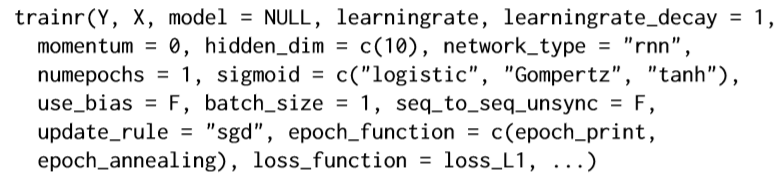
\includegraphics[width=0.45\textwidth]{figure/rnn_package.png}
     \caption{Package rnn, CRAN}
\end{figure}
\paragraph{Pros}
\begin{itemize}
\item Allows to run a demonstration of how RNN models work by using predefined values and allowing the user to see the impact of a changes in the model's hyperparameters by using the function \textbf{run.rnn\_demo()}
\item Allows to plot the model's errors through all epochs.
\item Allows to use LSTM and GRU models.
\end{itemize}
\paragraph{Cons}
\begin{itemize}
\item Uses R native, therefore it might not be the best package in terms of time computation.
\end{itemize}

%%%%%%%%%%%%%%%%%%%%%%%%%%%%%%%%%%%%%%%%%%%%%%%%%%%
%%%%%%%%%%%%%%%%%%  API  %%%%%%%%%%%%%%%%%%%%%%%%%%
%%%%%%%%%%%%%%%%%%%%%%%%%%%%%%%%%%%%%%%%%%%%%%%%%%%
\subsection{API packages}

%%%%%%%%%%%%%%%% Keras %%%%%%%%%%%%%%%% 
\subsubsection{Keras}
\textbf{Keywords: FNN, CNN, RNN}
\paragraph{Description}
This API is really popular in the Python world because it acts like a wrapper of more popular libraries. It might become hard to follow but Keras has multiple backends such as Tensorflow, Theano and MXNET. The \textit{Keras} \cite{keras2019} is mostly use to link the wrapper tool with R. The most useful reference one can get for this workflow is written by two major players ; \textit{Keras} creator and \textit{RStudio} creator. It explains in detail the best practices in order to use \textit{Keras} in R \cite{chollet2018deep}.

\paragraph{Pros}
\begin{itemize}
\item Give a lot of flexibility since can basically be use to create all type of deep learning algorithms.
\item Easy and fast prototyping
\item Construct models exactly the same way as in python with a minimalist philosphy.
\item Give the possibility to save everything on the workspace (model, training history, etc.)
\end{itemize}
\paragraph{Cons}
\begin{itemize}
\item It is an encapsulation of a program inside a python environment.
\item For some, it might be to high level and limit the customization.
\item It can only work on top Tensorflow, CNTK and Theano backend.
\end{itemize}

%%%%%%%%%%%%%%%% Tensorflow %%%%%%%%%%%%%%%% 
\subsubsection{Tensorflow}
\textbf{Keywords: FNN, CNN, RNN}
\paragraph{Description}
This library was created by Google and written in $C++$ and python. It is pretty well known in the python enviromnent. Recently, a R package was created to interface this popular library \cite{tensorflow2019}."'TensorFlow' was originally developed by researchers and engineers working on the Google Brain Team within Google's Machine Intelligence research organization for the purposes of conducting machine learning and deep neural networks research."
\paragraph{Pros}
\begin{itemize}
\item Well documented with a lot of tutorials online.
\item Pre trained models accessible
\end{itemize}

\paragraph{Cons}
\begin{itemize}
\item Struggles with poor results for speed.
\item Not a trivial since it is consider a low-level coding
\end{itemize}

%%%%%%%%%%%%%%%% MXNET %%%%%%%%%%%%%%%% 
\subsubsection{MXNet}
\textbf{Keywords: FNN, CNN, RNN}
\paragraph{Description}
MXNet is a DL framework open source created by Apache. The framework is mostly backed by Intel, Microsoft and MIT. There is a manual\cite{mxnet2020} but itsn't part of the CRAN database.
\paragraph{Pros}
\begin{itemize}
\item Allows the use of multiple CPU and multiple GPU, but it requires to download the package Rtools and a c++ compiler.
\item Very easy to use and has a flexible implementation of diffenent neural networks architectures and models.
\item The models can be built layer per layer.
\item Provide details and information about the learning progress during the training phase.
\end{itemize}
\paragraph{Cons}
\begin{itemize}
\item It has a smaller community compared to other popular framework.
\item A package more use in the industrial projects and not so much in the research community.
\end{itemize}


%%%%%%%%%%%%%%%% rTorch %%%%%%%%%%%%%%%% 
\subsubsection{rTorch}
The rTorch CRAN package is to interface the popular open source machine learning library PyTorch\cite{rTorch2019}. The PyTorch was developed by Facebook AI Research lab (FAIR) and all the original features are available in rTorch.

\paragraph{Description}
\paragraph{Pros}
\begin{itemize}
\item Multiple pre-trained model available 
\item Simple and easy to use 
\end{itemize}
\paragraph{Cons}
\begin{itemize}
\item It is an encapsulation of a program inside a python environment.
\end{itemize}
%%%%%%%%%%%%%%%% H2o %%%%%%%%%%%%%%%% 
\subsubsection{H2o}
\paragraph{Description}
H2o is a "scalable open source machine learning platform that offers parallelized implementations of many supervised, unsupervised and fully automatic machine learning algorithms on clusters". This package allows to run H2o via its REST API through R and offers several advantages such as the ability ot know the computation time remaining when running a model.
\begin{figure}[h]
    \centering
    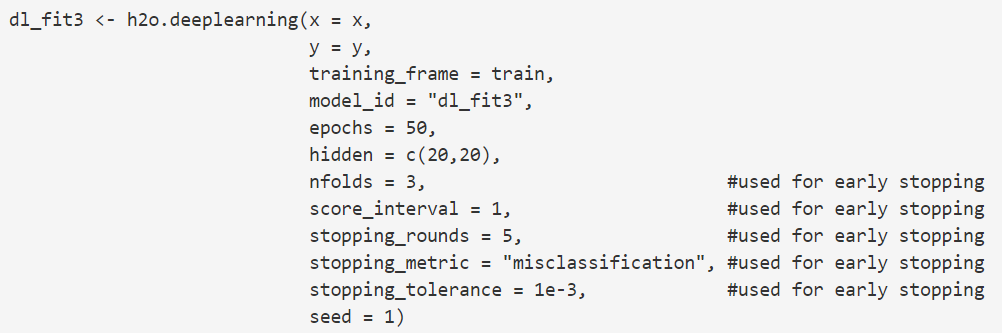
\includegraphics[width=0.65\textwidth]{figure/h2o_package.png}
     \caption{H2o package}
\end{figure}

\paragraph{Pros}
\begin{itemize}
\item Very easy to use and includes a cross-validation feature and functions for grid search in order to optimize the model's hyperparameters.
\item 
\item Allows the use of multiple CPU.
\item Provide an adaptive learning rate (ADADELTA) which improves the optimization process by having a different learning rate for each neuron.
\item Provide details and information about the learning progress during the training phase.
\item Really fast computation training
\end{itemize}
\paragraph{Cons}
\begin{itemize}
\item Requires the latest version of Java.
\item The deep learning package has a huge amount of parameters, however, it doesn't give all the capability of other resources.
\end{itemize}

%%%%%%%%%%%%%%%%%%%%%%%%%%%%%%%%%%%%%%%%%%%%%%%%%%%
%%%%%%%%%%%%%%%%%% Examples    %%%%%%%%%%%%%%%%%%%%
%%%%%%%%%%%%%%%%%%%%%%%%%%%%%%%%%%%%%%%%%%%%%%%%%%%
\section{Examples}
\label{sec:examples}
In order to give concrete deep learning examples, four resources were selected for tutorials; Keras using Tensorflow backend, H2O, rTorch and MXNET.

%%%%%%%%%%%%%%%% Keras %%%%%%%%%%%%%%%% 
\subsection{Keras}
\subsubsection{Installation}
First step, is the installation and download of the Keras files from GitHub :
\begin{knitrout}
\definecolor{shadecolor}{rgb}{0.969, 0.969, 0.969}\color{fgcolor}\begin{kframe}
\begin{alltt}
\hlstd{devtools}\hlopt{::}\hlkwd{install_github}\hlstd{(}\hlstr{"rstudio/keras"}\hlstd{)}
\end{alltt}
\end{kframe}
\end{knitrout}
Then, we need to to install the package and import in the project :
\begin{knitrout}
\definecolor{shadecolor}{rgb}{0.969, 0.969, 0.969}\color{fgcolor}\begin{kframe}
\begin{alltt}
\hlkwd{library}\hlstd{(keras)}
\hlkwd{install_keras}\hlstd{()}
\end{alltt}
\end{kframe}
\end{knitrout}
When the "\textit{Installation complete.}" message appear you have a complete installation with CPU configure on the TensorFlow backend.
If you want to take advantage of your GPU (Ensure that you have the hardware prerequisites) you will need to execute a different command as follows:
\begin{knitrout}
\definecolor{shadecolor}{rgb}{0.969, 0.969, 0.969}\color{fgcolor}\begin{kframe}
\begin{alltt}
\hlkwd{install_keras}\hlstd{(}\hlkwc{tensorflow} \hlstd{=} \hlstr{"gpu"}\hlstd{)}
\end{alltt}
\end{kframe}
\end{knitrout}
\subsubsection{FNN}
\begin{knitrout}
\definecolor{shadecolor}{rgb}{0.969, 0.969, 0.969}\color{fgcolor}\begin{kframe}
\begin{alltt}
\hlkwd{library}\hlstd{(keras)}

\hlcom{# create model}
\hlstd{model_keras} \hlkwb{=} \hlkwd{keras_model_sequential}\hlstd{()}
\hlstd{model_keras} \hlopt
  \hlkwd{layer_dense}\hlstd{(}\hlkwc{units} \hlstd{=} \hlnum{8}\hlstd{,} \hlkwc{activation} \hlstd{=} \hlstr{'relu'}\hlstd{,} \hlkwc{input_shape} \hlstd{=} \hlkwd{c}\hlstd{(}\hlnum{4}\hlstd{))} \hlopt
  \hlkwd{layer_dense}\hlstd{(}\hlkwc{units} \hlstd{=} \hlnum{3}\hlstd{,} \hlkwc{activation} \hlstd{=} \hlstr{'softmax'}\hlstd{)}
\hlcom{# Compile model}
\hlstd{model_keras} \hlopt \hlkwd{compile}\hlstd{(}
  \hlkwc{loss} \hlstd{=} \hlstr{'categorical_crossentropy'}\hlstd{,}
  \hlkwc{optimizer} \hlstd{=} \hlkwd{optimizer_adam}\hlstd{(),}
  \hlkwc{metrics} \hlstd{=} \hlkwd{c}\hlstd{(}\hlstr{'accuracy'}\hlstd{)}
\hlstd{)}
\hlstd{start_time} \hlkwb{<-} \hlkwd{Sys.time}\hlstd{()}
\hlstd{history} \hlkwb{<-} \hlstd{model_keras} \hlopt \hlkwd{fit}\hlstd{(}
  \hlkwd{as.matrix}\hlstd{(X}\hlopt{$}\hlstd{train),}\hlkwd{to_categorical}\hlstd{(Y}\hlopt{$}\hlstd{train),}
   \hlkwc{epochs}\hlstd{=}\hlnum{200}\hlstd{,} \hlkwc{batch_size}\hlstd{=}\hlnum{5}\hlstd{)}
\hlstd{end_time} \hlkwb{<-} \hlkwd{Sys.time}\hlstd{()}

\hlcom{#Benchmark}
\hlstd{time_fnn_keras} \hlkwb{=} \hlstd{end_time} \hlopt{-} \hlstd{start_time}
\hlstd{model_keras} \hlopt \hlkwd{evaluate}\hlstd{(X}\hlopt{$}\hlstd{test,} \hlkwd{to_categorical}\hlstd{(Y}\hlopt{$}\hlstd{test))}
\hlstd{model_keras} \hlopt \hlkwd{predict}\hlstd{(X}\hlopt{$}\hlstd{test,} \hlkwd{to_categorical}\hlstd{(Y}\hlopt{$}\hlstd{test))}

\hlstd{preds} \hlkwb{=} \hlkwd{predict}\hlstd{(model_keras,}\hlkwd{as.array}\hlstd{(X}\hlopt{$}\hlstd{test))}
\hlstd{pred.label.keras} \hlkwb{<-} \hlkwd{max.col}\hlstd{((preds))} \hlopt{-} \hlnum{1}
\hlnum{1}\hlopt{-}\hlkwd{mean}\hlstd{(pred.label.keras} \hlopt{!=} \hlkwd{as.vector}\hlstd{(data_df}\hlopt{$}\hlstd{test}\hlopt{$}\hlstd{Species))}
\end{alltt}
\end{kframe}
\end{knitrout}

This package of the possibility to store the training history :
\begin{knitrout}
\definecolor{shadecolor}{rgb}{0.969, 0.969, 0.969}\color{fgcolor}\begin{kframe}
\begin{alltt}
\hlkwd{plot}\hlstd{(history)}
\end{alltt}


{\ttfamily\noindent\itshape\color{messagecolor}{\#\# `geom\_smooth()` using formula 'y \textasciitilde{} x'}}\end{kframe}
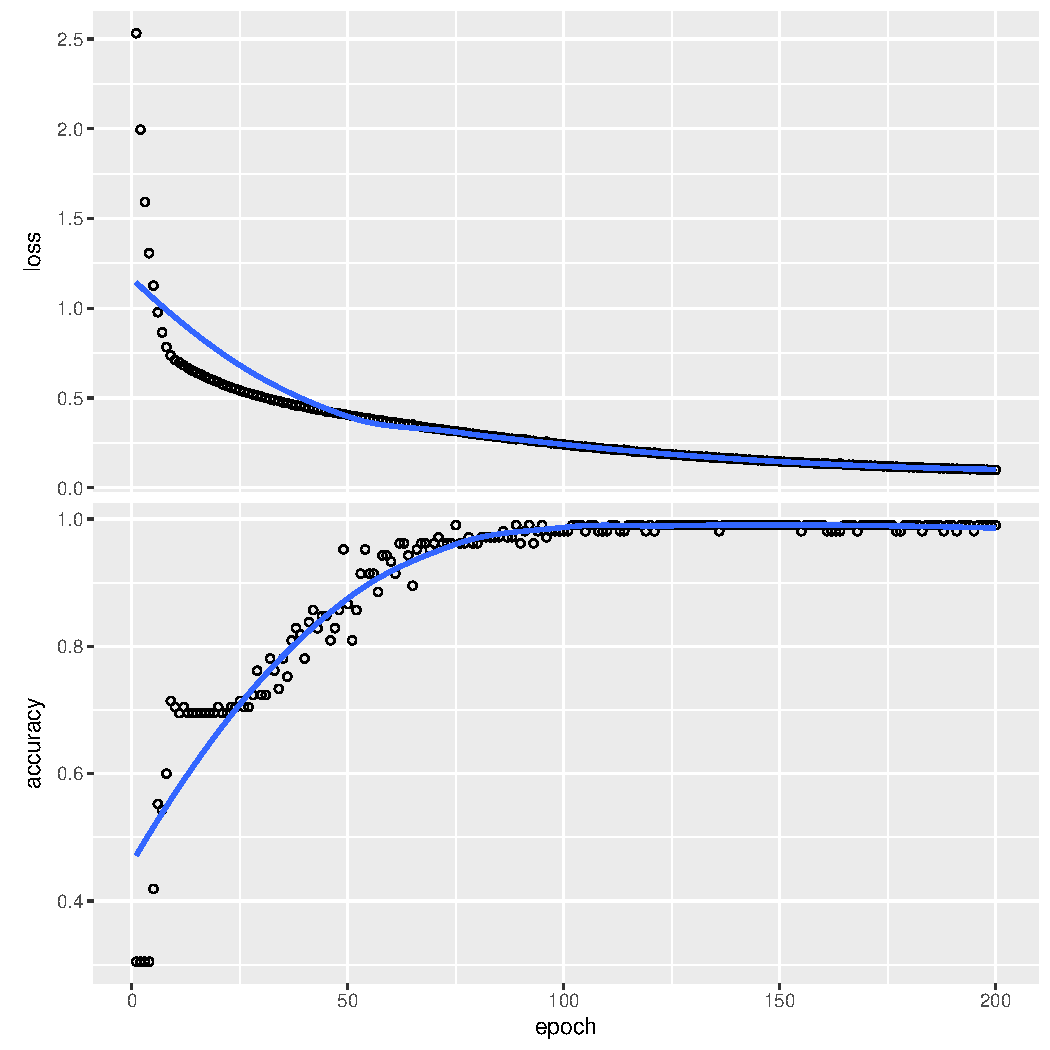
\includegraphics[width=4in]{figure/unnamed-chunk-10-1} 

\end{knitrout}

The accuracy of this resources is
\begin{knitrout}
\definecolor{shadecolor}{rgb}{0.969, 0.969, 0.969}\color{fgcolor}\begin{kframe}
\begin{verbatim}
## [1] 0.9333333
\end{verbatim}
\end{kframe}
\end{knitrout}
and the time it took to train is :
\begin{knitrout}
\definecolor{shadecolor}{rgb}{0.969, 0.969, 0.969}\color{fgcolor}\begin{kframe}
\begin{verbatim}
## Time difference of 1.213505 mins
\end{verbatim}
\end{kframe}
\end{knitrout}

\subsubsection{CNN}
\subsubsection{RNN}

%%%%%%%%%%%%%%%% H2o %%%%%%%%%%%%%%%% 
\subsection{H2O}
\subsubsection{Installation}
\begin{knitrout}
\definecolor{shadecolor}{rgb}{0.969, 0.969, 0.969}\color{fgcolor}\begin{kframe}
\begin{alltt}
\hlkwd{install.packages}\hlstd{(}\hlstr{"h2o"}\hlstd{)}
\hlkwd{library}\hlstd{(h2o)}
\hlkwd{h2o.init}\hlstd{()}
\end{alltt}
\end{kframe}
\end{knitrout}
By default, H2O Deep Learning uses an adaptive learning rate (ADADELTA) for its stochastic gradient descent optimization.
\textbf{Prerequisites to launch H2o}, 64 bit Java 6+ if you want to open a h2o model that s more than 1 GB. 
\subsubsection{FNN}
\begin{knitrout}
\definecolor{shadecolor}{rgb}{0.969, 0.969, 0.969}\color{fgcolor}\begin{kframe}
\begin{alltt}
\hlkwd{library}\hlstd{(h2o)}
\hlkwd{h2o.init}\hlstd{()}
\hlcom{# Identify predictors and response}


\hlstd{h2o_df_train} \hlkwb{=} \hlkwd{as.h2o}\hlstd{(data_df}\hlopt{$}\hlstd{train)}
\hlstd{h2o_df_test} \hlkwb{=} \hlkwd{as.h2o}\hlstd{(data_df}\hlopt{$}\hlstd{test)}

\hlstd{y} \hlkwb{<-} \hlstr{"Species"}
\hlstd{x} \hlkwb{<-} \hlkwd{setdiff}\hlstd{(}\hlkwd{names}\hlstd{(h2o_df_train), y)}
\hlcom{# For binary classification, response should be a factor}
\hlstd{h2o_df_train[,y]} \hlkwb{<-} \hlkwd{as.factor}\hlstd{(h2o_df_train[,y])}
\hlstd{h2o_df_test[,y]} \hlkwb{<-} \hlkwd{as.factor}\hlstd{(h2o_df_test[,y])}

\hlstd{start_time} \hlkwb{<-} \hlkwd{Sys.time}\hlstd{()}
\hlstd{model_h2o} \hlkwb{<-} \hlkwd{h2o.deeplearning}\hlstd{(}\hlkwc{x} \hlstd{= x,}
                              \hlkwc{y} \hlstd{= y,}
                              \hlkwc{training_frame} \hlstd{= h2o_df_train,}
                              \hlkwc{epochs} \hlstd{=} \hlnum{200}\hlstd{,}
                              \hlkwc{seed}\hlstd{=}\hlnum{123}\hlstd{)}
\hlstd{end_time} \hlkwb{<-} \hlkwd{Sys.time}\hlstd{()}
\hlstd{time_fnn_h2o} \hlkwb{=} \hlstd{end_time} \hlopt{-} \hlstd{start_time}

\hlkwd{summary}\hlstd{(model_h2o)}

\hlstd{perf} \hlkwb{<-} \hlkwd{h2o.performance}\hlstd{(model_h2o,} \hlkwd{as.h2o}\hlstd{(data_df}\hlopt{$}\hlstd{test))}
\hlstd{pred} \hlkwb{<-} \hlkwd{h2o.predict}\hlstd{(model_h2o,} \hlkwd{as.h2o}\hlstd{(data_df}\hlopt{$}\hlstd{test))}
\hlnum{1}\hlopt{-}\hlkwd{mean}\hlstd{(}\hlkwd{as.vector}\hlstd{(pred}\hlopt{$}\hlstd{predict)} \hlopt{!=} \hlkwd{as.vector}\hlstd{(data_df}\hlopt{$}\hlstd{test}\hlopt{$}\hlstd{Species))}
\end{alltt}
\end{kframe}
\end{knitrout}
The accuracy of this resources is
\begin{knitrout}
\definecolor{shadecolor}{rgb}{0.969, 0.969, 0.969}\color{fgcolor}\begin{kframe}
\begin{verbatim}
## [1] 0.9333333
\end{verbatim}
\end{kframe}
\end{knitrout}
and the time it took to train is :
\begin{knitrout}
\definecolor{shadecolor}{rgb}{0.969, 0.969, 0.969}\color{fgcolor}\begin{kframe}
\begin{verbatim}
## Time difference of 7.731083 secs
\end{verbatim}
\end{kframe}
\end{knitrout}
\subsubsection{CNN}
\subsubsection{RNN}


%%%%%%%%%%%%%%%% MXNET %%%%%%%%%%%%%%%% 
\subsection{MXNET}
\subsubsection{Installation}
For CPU :
\begin{knitrout}
\definecolor{shadecolor}{rgb}{0.969, 0.969, 0.969}\color{fgcolor}\begin{kframe}
\begin{alltt}
\hlkwd{install.packages}\hlstd{(}\hlstr{"https://s3.ca-central-1.amazonaws.com/jeremiedb/share/mxnet/CPU/mxnet.zip"}\hlstd{,}
                 \hlkwc{repos} \hlstd{=} \hlkwa{NULL}\hlstd{)}
\hlkwd{library}\hlstd{(mxnet)}
\end{alltt}
\end{kframe}
\end{knitrout}

\subsubsection{FNN}
\begin{knitrout}
\definecolor{shadecolor}{rgb}{0.969, 0.969, 0.969}\color{fgcolor}\begin{kframe}
\begin{alltt}
\hlkwd{install.packages}\hlstd{(}\hlstr{"https://s3.ca-central-1.amazonaws.com/jeremiedb/share/mxnet/CPU/mxnet.zip"}\hlstd{,} \hlkwc{repos} \hlstd{=} \hlkwa{NULL}\hlstd{)}
\hlkwd{library}\hlstd{(mxnet)}
\hlstd{data} \hlkwb{<-} \hlkwd{mx.symbol.Variable}\hlstd{(}\hlstr{"data"}\hlstd{)}
\hlstd{fc1} \hlkwb{<-} \hlkwd{mx.symbol.FullyConnected}\hlstd{(data,} \hlkwc{name}\hlstd{=}\hlstr{"fc1"}\hlstd{,} \hlkwc{num_hidden}\hlstd{=}\hlnum{8}\hlstd{)}
\hlstd{act1} \hlkwb{<-} \hlkwd{mx.symbol.Activation}\hlstd{(fc1,} \hlkwc{name}\hlstd{=}\hlstr{"relu1"}\hlstd{,} \hlkwc{act_type}\hlstd{=}\hlstr{"relu"}\hlstd{)}
\hlstd{fc2} \hlkwb{<-} \hlkwd{mx.symbol.FullyConnected}\hlstd{(act1,} \hlkwc{name}\hlstd{=}\hlstr{"fc2"}\hlstd{,} \hlkwc{num_hidden}\hlstd{=}\hlnum{3}\hlstd{)}
\hlstd{softmax} \hlkwb{<-} \hlkwd{mx.symbol.SoftmaxOutput}\hlstd{(fc2,} \hlkwc{name}\hlstd{=}\hlstr{"sm"}\hlstd{)}
\hlkwd{mx.set.seed}\hlstd{(}\hlnum{123}\hlstd{)}

\hlstd{start_time} \hlkwb{<-} \hlkwd{Sys.time}\hlstd{()}
\hlstd{model_mx} \hlkwb{<-} \hlkwd{mx.model.FeedForward.create}\hlstd{(}
  \hlstd{softmax,}
  \hlkwc{X}\hlstd{=}\hlkwd{as.array}\hlstd{(X}\hlopt{$}\hlstd{train),}
  \hlkwc{y}\hlstd{=}\hlkwd{as.numeric}\hlstd{(Y}\hlopt{$}\hlstd{train),}
  \hlkwc{ctx}\hlstd{=}\hlkwd{mx.cpu}\hlstd{(),}
  \hlkwc{num.round}\hlstd{=}\hlnum{200}\hlstd{,}
  \hlkwc{verbose} \hlstd{=} \hlnum{TRUE}\hlstd{,}
  \hlkwc{eval.metric} \hlstd{= mx.metric.accuracy,}
  \hlkwc{array.batch.size}\hlstd{=}\hlnum{5}\hlstd{)}
\hlstd{end_time} \hlkwb{<-} \hlkwd{Sys.time}\hlstd{()}
\hlstd{time_fnn_mxnet} \hlkwb{=} \hlstd{end_time} \hlopt{-} \hlstd{start_time}


\hlstd{preds} \hlkwb{=} \hlkwd{predict}\hlstd{(model_mx,}\hlkwd{as.array}\hlstd{(X}\hlopt{$}\hlstd{test),}\hlkwc{array.layout} \hlstd{=} \hlstr{"rowmajor"}\hlstd{)}
\hlkwd{summary}\hlstd{(model_mx)}
\hlstd{pred.label.mxnet} \hlkwb{<-} \hlkwd{max.col}\hlstd{(}\hlkwd{t}\hlstd{(preds))} \hlopt{-} \hlnum{1}
\hlnum{1}\hlopt{-}\hlkwd{mean}\hlstd{(pred.label.mxnet} \hlopt{!=} \hlkwd{as.vector}\hlstd{(data_df}\hlopt{$}\hlstd{test}\hlopt{$}\hlstd{Species))}
\end{alltt}
\end{kframe}
\end{knitrout}
The accuracy of this resources is
\begin{knitrout}
\definecolor{shadecolor}{rgb}{0.969, 0.969, 0.969}\color{fgcolor}\begin{kframe}
\begin{verbatim}
## [1] 0.9333333
\end{verbatim}
\end{kframe}
\end{knitrout}
and the time it took to train is :
\begin{knitrout}
\definecolor{shadecolor}{rgb}{0.969, 0.969, 0.969}\color{fgcolor}\begin{kframe}
\begin{verbatim}
## Time difference of 6.597001 secs
\end{verbatim}
\end{kframe}
\end{knitrout}
\subsubsection{CNN}
\subsubsection{RNN}

%%%%%%%%%%%%%%%%%%%%%%%%%%%%%%%%%%%%%%%%%%%%%%%%%%%
%%%%%%%%%%%%%%%%%% Discussion  %%%%%%%%%%%%%%%%%%%%
%%%%%%%%%%%%%%%%%%%%%%%%%%%%%%%%%%%%%%%%%%%%%%%%%%%
\section{Discussion}

%%%%%%%%%%%%%%%%%%%%%%%%%%%%%%%%%%%%%%%%%%%%%%%%%%%
%%%%%%%%%%%%%%%%%% Biblio      %%%%%%%%%%%%%%%%%%%%
%%%%%%%%%%%%%%%%%%%%%%%%%%%%%%%%%%%%%%%%%%%%%%%%%%%
\newpage
\pagestyle{plain}
\bibliography{global.bib}
\end{document}
